\section [Clogging simulation (2D)]{2D reactive transport simulation of COMEDY clogging experiment}
\label{benchmark_2d_comedy}

Clogging is a widely occurring phenomena in the porous media. The change of pore space structure normally leads to different behaviors of hydraulics. In such systems, flow and transport of solutes are strongly coupled with chemical reactions, imposing challenges to numerical simulations. The COMEDY experimental setup \cite{Cochepin2008} was a 2D reactive transport scenario which involves clogging and perforation of an interface. Numerical models such as CRUNCH and HYTECH have been applied to simulate it. In this section, simulation results from OpenGeoSys-GEM are compared against those from other codes. 

\subsection{Definition}
\ref{hc:comedy_domain} shows the geometry of the model domain. It is a chamber containing 3 regions. Two of them (Q1 and Q3) are made of chemically inert quartz and the central region (Q2) contains the reactant mineral portlandite. Oxalate ions were injected as a constant flux through Inlet 2, and sodium chloride solutions were introduced through Inlet 1. In Q2, the chemical reaction between the inlet solution and portlandite leads to the precipitation of calcium oxalate, as in the following. 
\begin{equation}
\label{eq:CaOxylate}
C_2O_4^{2-} + Ca(OH)_2 + H_2O \Rightarrow CaC_2O_4 \cdot H2O + 2OH^-
\end{equation} 

\begin{figure}[!htb]
  \begin{center}
  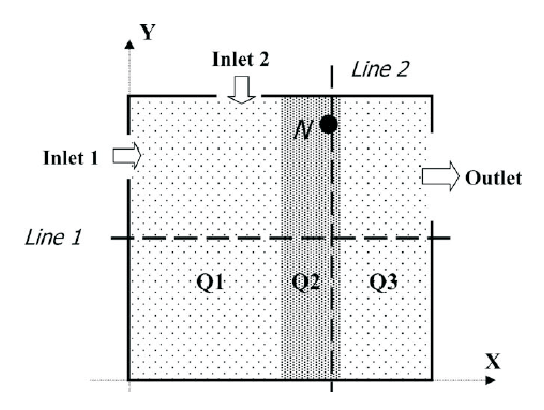
\includegraphics[scale=1.0]{PART_III/HC/comedy_domain.eps}
  \end{center}
  \caption{2D model domain for the COMEDY experiment according to \cite{Cochepin2008}. The setup is a square (14 cm of edge size). Lines labeled Line 1 (y = 7.0 cm) and Line 2 (x = 9.5 cm) (respectively node N (x = 9.5 cm; y = 10.8 cm)) are test lines/node on which specific profiles will be compared.}
  \label{hc:comedy_domain}
\end{figure}

The initial and boundary chemical was set up using the GEMS-PSI software package. It implements a Gibbs energy minimization algorithm in thermodynamic modeling of equilibrium in heterogeneous aquatic chemical systems. The oxalate ion was introduced as an independent component in the thermodynamic database. The reaction \ref{eq:CaOxylate} was also introduced with equivalent logK values as in \cite{Cochepin2008}. The detailed chemical set up for the different regions are given in \ref{tab:comedy_gems_sys}. At some points, the system is in an undefined redox state. To avoid this, a small amount of dissolved $O_2$ was introduced in the initial bulk composition to keep the system in oxic condition. The value of porosity is obtained using the ratio $V_{Initial} / V_{Total}$. 

% Table of chemical system. 
\begin{table}[h]
\caption{Equilibrium amount of independent components and phases for boundary and initial conditions}
\begin{tabular}{p{2cm}lllll}
\hline
\multirow{10}{2cm}{Amount of chemical species in aqueous phase (mol)}
  & Component & Q1(=Q3) & Q2      & I1      & I2      \\
\hline
  & C         & 1.00e-5 & 5.50e-8 & 6.20e-8 & 5.51e-8 \\
  & Ca        & 1.00e-5 & 3.32    & 4.70e-8 & 3.00e-8 \\
  & Cl        & 1.20e-5 & 1.71e-12& 0.02    & 4.25e-5 \\
  & H         & 33.2    & 27.7    & 33.2    & 33.3    \\
  & Na        & 1.71e-10& 1.35e-3 & 0.02    & 0.8     \\
  & O         & 78.3    & 78.9    & 78.3    & 78.4    \\
  & Oxa       & 2.00e-8 & 1.00e-8 & 2.00e-8 & 0.40    \\
  & Si        & 30.9    & 30.9    & 30.9    & 30.9    \\
  & Zz        & 0       & 0       & 0       & 0       \\
\hline
\multirow{7}{2cm}{Amount of solid phases (mol)}
  & Graphite  & 3.50e-8 & 3.50e-8 & 3.50e-8 & 3.50e-8 \\
  & Aragonite & 1.00e-8 & 1.00e-8 & 1.70e-8 & 1.00e-8 \\ 
  & Calcite   & 1.00e-5 & 1.00e-8 & 1.00e-8 & 1.00e-8 \\
  &Portlandite& 0       & 3.33    & 0       & 0       \\
  &Calcium Oxalate&1.00e-8&1.00e-8&1.00e-8  &1.00e-8  \\
  &Quartz     & 30.87   & 30.87   & 30.87   & 30.87   \\
  &Amorph Silica& 0     & 0       & 0       & 0       \\
\hline
\multirow{2}{2cm}{Equilibrium state}
  &pH         & 7       & 12.5    & 7       & 7       \\
  &Liquid volume (L)&0.3& 0.19    & 0.3     & 0.3     \\
  &Total volume  (L)&1  & 1       & 1       & 1       \\
\hline
\end{tabular}
\label{tab:comedy_gems_sys}
\end{table}

The chamber is discretized with a finite element mesh of quadrilateral elements of 3.3 mm size. The domain contains 1849 nodes and 1764 elements. A variable time step scheme is used to calculate the maximal time step size, which influences the accuracy of simulation result. 

The pressure at the outlet is set to 1 Bar.
\begin{table}[h]
\caption{Hydraulic parameters of the model domain}
\begin{center}
\begin{tabular}{lccc}
\hline
Parameters                       & Q1      & Q2      &  Q3      \\
\hline
Hydraulic conductivity ($m^2/s$) & 1.00e-5 & 1.64e-6 &  1.00e-5 \\
Dispersivity ($m$)               & 2.00e-2 & 2.00e-2 &  2.00e-2 \\
Diffusion coefficient ($m^2/s $) & 3.33e-9 & 3.33e-9 &  3.33e-9 \\
Tortuosity                       & 1.0     & 1.58    &  1.0     \\
\hline
\end{tabular}
\label{tab:comedy_H_par}
\end{center}
\end{table}

The tortuosity is set different for Q2 region to mimic the initial effective diffusion coefficient, which is the same ($1\times 10^{-09}$) for the 3 regions in \cite{Cochepin2008}. 
\begin{table}[h]
\caption{Model Setup for the inlets}
\begin{tabular}{l|c|c}
\hline
Velocity (m/s)  & Inlet 1    & Inlet 2    \\
\hline
x               & 5.7143e-10 & 0          \\
y               & 0          & 11.429e-10 \\
\hline
\end{tabular}
\label{tab:comedy_inlet}
\end{table}
In this study diffusion and dispersion are assumed isotropic and $D^*$ reduces to a scalar form, $D* = \alpha \| \overrightarrow{U} \| + D$ where $D$ is the effective diffusion coefficient. It is assumed that all solutes have the same value. $\alpha$ (m) is the dispersivity of the porous medium and $\overrightarrow{U}$ is the Darcy velocity vector. In this benchmark, advection and diffusion govern the transport process. The Archie's diffusion law $D_e = n^m \cdot D_p$ is applied in this model. The dissolution/precipitation reaction rate $r_s$ (mol/s) )is defined according to the following formula, 

\begin{equation}
r_s = - A_s k_{rate}[ 1 - (Q_s / K) ]
\end{equation}
where $k_{rate}$ is the dissolution and precipitation rate constant ($mol \cdot m^2 \cdot s^{-1}$). $Q_s$ is the ion activity product. $K$ is the equilibrium constant and $A_s$ is the specific surface area ($m^2 \cdot mol^{-1}$). The values used here are $A_{bulk} = 1000 m^2_{solid} / m^3_{porous medium}$, $log_{10}K_{Portlandite} = -5$ and $log_{10}K_{CaOxa} = -5$. 

\subsection{Solution}
For the flow part, \ref{hc:comedy_flow_field} shows the Darcy velocities on Line 1, compared against the results given by HYTEC. The results obtained with OpenGeosys are in good accordance quantitatively and qualitatively.

\begin{figure}[!htb]
  \begin{center}
  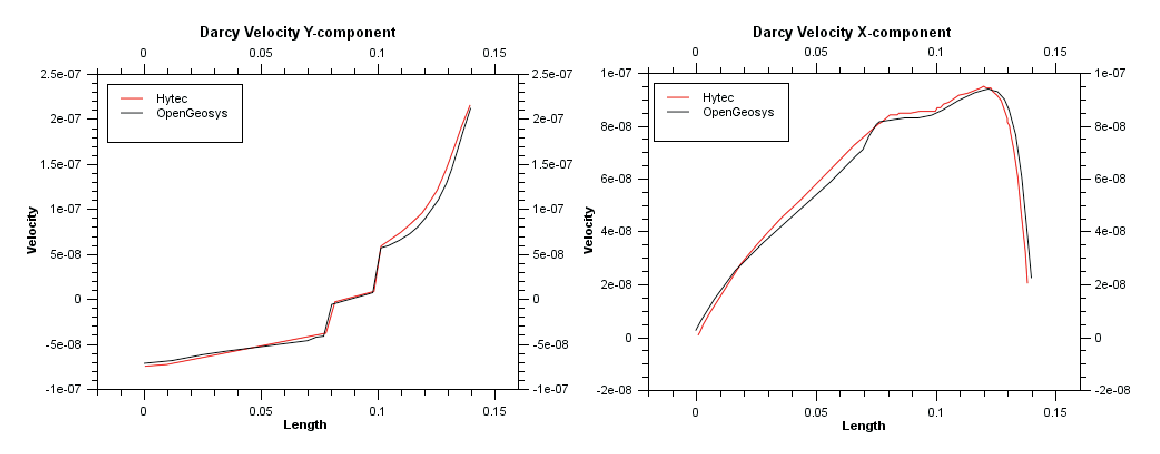
\includegraphics[scale=1.0]{PART_III/HC/comedy_flow.eps}
  \end{center}
  \caption{Darcy velocity profile on line 1 (x=70 cm)}
  \label{hc:comedy_flow_field}
\end{figure}

For the clogging process, porosity evolution profile \ref{hc:comedy_clogging} calculated by OpenGeoSys-GEM is compared against those from HYTEC and CRUNCH \cite{Cochepin2008}. Qualitatively the results are in good accordance. Portlandite dissolves and calcium oxalate precipitates. After the calcium oxalate volume fraction reaches a maximum it dissolves. The porosity follows the opposite evolution of mineral volume fraction due to the decrease of 33mL per mol of reacted portlandite. When calcium oxalate starts to dissolve, the porosity increases until it reaches the maximal value of 0.3 due to inert quartz background in Q2. 

Quantitatively, the results are different in several aspects. One of them is the evolution of porosity in time. With OpenGeosys, the portlandite dissolves much faster. It took 20 days in OGS whereas in CRUNCH and HYTEC the complete dissolution happens after 60 and 27 days respectively. The calcium oxalate is completely dissolved after 156 days in the OGS result, and took 60 and 90 days for CRUNCH and HYTEC. The porosity follows the same evolution in time. The dissolution time of calcium oxalate can slightly be reduced by increasing its precipitation/dissolution rate. Another difference is that with HYTEC and CRUNCH, portlandite volume ratio remain approximatively constant for the 20 days before dissolving. This difference can be explained by the fact that water in Q1 and Q3 is not in equilibrium with portlandite. When it diffuses into Q2, it starts to dissolve portlandite before oxalate ions reach the node N. Also noticed is, the hight of the maximum of calcium oxalate (20\% vol. for Opengeosys, 28.1\% vol. for Crunch, and 25.5\% vol. for Hytec) makes the obstacle created with the OpenGeosys simulation more permeable. An increase in the hight of the maximum is observed when the precipitation/dissolution rate of calcium oxalate is increased. 

\begin{figure}[!htb]
  \begin{center}
  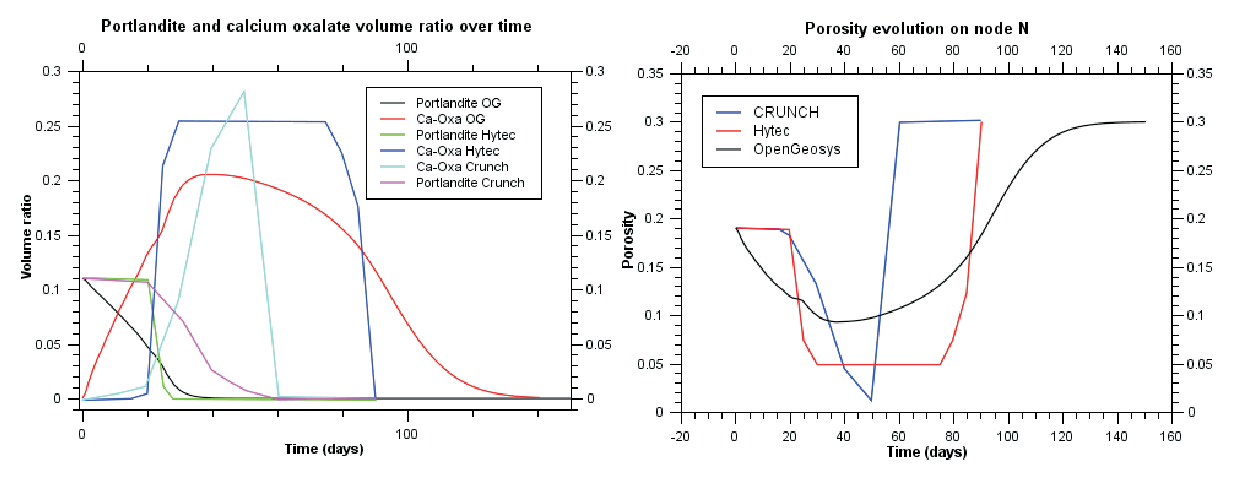
\includegraphics[scale=0.4]{PART_III/HC/comedy_porosity.eps}
  \end{center}
  \caption{Solids volume ratio and porosity evolution on node N (x=0.096m ; y=0.11m)}
  \label{hc:comedy_clogging}
\end{figure}




